\chapter{Grundlagen Neuronaler Feedforward Netze}
\label{ch:mlp}
Neuronale Netze sind äußerst vielseitig. Inspiriert von Gehirnen von Lebewesen, die  einem komplexen, nichtlinearen, parallelen Computer ähneln, finden sie heute Anwendung in der Modellierung, Zeitreihenanalyse, Mustererkennung und Signalverarbeitung. Eine sehr wichtige Eigenschaft ist hierbei die Möglichkeit, von Eingabedaten beziehungsweise Trainingsdaten überwacht, unüberwacht und bekräftigend zu lernen \cite[vgl.][S. 1]{Haykin1999}. Dies erlaubt einen universellen Einsatz in allen Teilgebieten des maschinellen Lernens (vgl. Kapitel \ref{ch:Einleitung}).
Grundsätzlich werden drei Typen neuronaler Netze unterschieden: \textit{Single-Layer Feedforward Networks}, \textit{Multilayer Feedforward Networks} und \textit{Recurrent Networks} \cite[vgl.][S. 22f]{Haykin1999}. Diese Arbeit beschränkt sich jedoch auf nicht rekurrente \textit{Multilayer Feedforward Networks} in den Bereichen Klassifikation und Regression und beschreibt somit das klassische überwachte, neuronale Lernmodell (siehe Kapitel \ref{ch:Einleitung}).


\section{Perzeptron und Multilayer Perceptron}
\begin{figure}
\centering
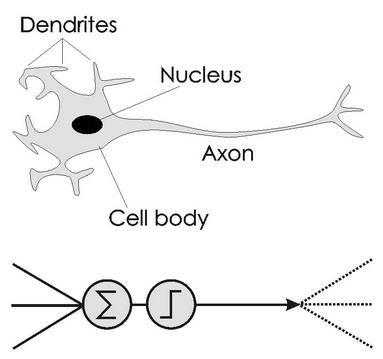
\includegraphics[width=0.4\linewidth]{images/2_neuron}
\caption[Schematischer Vergleich von biologischen und künstlichen \cite{McCulloch1943} Neuronen ]{Schematischer Vergleich von biologischen und künstlichen Neuronen von \cite{McCulloch1943} (nach \cite{Winston1992}, S. 444 ff.)}
\label{fig:2_Neuron}
\end{figure}
Heutige Neuronale Netze basieren auf dem in den späten 1950er von \cite{Rosenblatt1962} entwickelten Perzeptron. Wie Abbildung \ref{fig:2_Neuron} zeigt, ist die Architektur des Perzeptron an biologische Neuronen angelehnt. Die Ausgabe wird berechnet indem die Summe über die Produkte zwischen der Eingabe $x_i$ und den Gewichten $w_i$ gebildet wird. Erreicht die Summe einen definierten Schwellwert (\textit{Bias}) $-b$, wird das Neuron aktiviert und gibt die binäre Eins aus, ansonsten die binäre Null. Formal berechnet das Perzeptron somit die in Gleichung \ref{eq:perceptron} aufgeführte Funktion.
\begin{equation}
\label{eq:perceptron}
f(x) = sign(\sum_{i}^{n} w_ix_i + b) = sign(\langle w, x \rangle + b) 
\end{equation}

Obwohl das Perzeptron sich in dieser Form bereits als linearer Klassifikator eignet, ist es in seiner Ausdrucksstärke sehr eingeschränkt. So ist es beispielsweise nicht möglich Entscheidungshierarchien, wie in Netzwerken von \cite{McCulloch1943}, zu bilden und somit das bekannte XOR-Problem zu lösen.

Die Erweiterung zum Perzeptron stellt das in den 1980er Jahren von \cite{Rumelhart1986b} entwickelte \textit{Multilayer Perceptron} (MLP) dar. Die Architektur eines MLP wird bestimmt durch die Anzahl an Schichten (\textit{Layers}) sowie der pro Schicht enthaltenen Neuronen. Abbildung \ref{fig:2_mlp} zeigt die generische Organisation mehrerer Neuronen in der Eingabeschicht (Input-Layer), der Verdeckten Schicht (Hidden-Layer) und der Ausgabeschicht (Output-Layer). Neuronen verallgemeinern hierbei das Perzeptron insofern, dass diese die Schwellwert-Aktivierungsfunktion durch eine beliebige Funktion $\phi(\cdot)$ ersetzen können. Somit ermöglichen diese auf die reellen Zahlen $\mathbb{R}$ abzubilden. Darüber hinaus kann durch die Darstellung von Entscheidungshierarchien auch das XOR-Problem gelöst werden \cite[vgl.][S. 125]{Rojas1996}. 

Zusammenfassend lässt sich sagen, dass  durch die richtige Wahl der Architektur und Aktivierungsfunktion mit MLPs eine beliebige Funktion $f:\mathbb{R}^n \rightarrow \mathbb{R}^m $ beliebig genau approximiert werden kann, was durch das \textit{Universal Approximation Theorem} beschrieben ist. Die Schwierigkeit besteht jedoch darin, dass die zu approximierende Funktion lediglich durch Trainingsbeispiele gegeben ist und die Gewichte und Schwellwerte durch Training so angepasst werden müssen, dass neue Werte möglichst gut extrapoliert werden (Generalisierung) \cite[vgl.][S. 24 ff.]{Rojas1996}. 

 \begin{figure}[H]
 \centering
 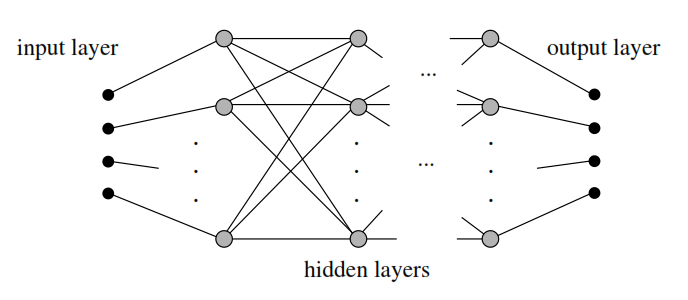
\includegraphics[width=0.8\linewidth]{images/2_mlp}
 \caption[Generische mehrschichtige Architektur eines MLP]{Generische mehrschichtige Architektur eines MLP (siehe \cite{Rojas1996}, S. 126)}
 \label{fig:2_mlp}
 \end{figure}

Ein einfaches Beispiel soll an dieser Stelle die Verbindung zwischen MLP und \textit{Deep Learning} herstellen. Die einfachste Architektur eines MLP umfasst die Eingabe $x$ (Eingabeneuronen), ein \textit{Hidden}-Neuron $w_2$ sowie ein Ausgabeneuron $w_1$. Formal wird diese Architektur durch die Funktion in Gleichung \ref{eq:deep_mlp} beschrieben, welche in unmittelbarer Verbindung zu den in Kapitel \ref{ch:DeepLearning} beschriebenen tiefen Architekturen steht.
\begin{equation}
\label{eq:deep_mlp}
f(x) = \phi(\langle w_1, \phi(\langle w_2, x \rangle + b_2) \rangle + b_1) 
\end{equation}

Analog dazu fusionieren die Gewichtsvektoren $w_i$ bei mehrere Neuronen in einer Schicht zu einer Matrix $ W $ in der die einzelnen $w_i$ der Neuronen zeilenweise organisiert sind. Das innere Produkt in der Gleichung \ref{eq:deep_mlp} wird so durch eine Matrix-Vektor-Multiplikation ersetzt und der skalare Schwellwert $b_i$ mit einem Vektor $b$. Eine Schicht eines MLP kann folglich mit $\phi(Wx + b)$ formal dargestellt werden.

\section{Aktivierungsfunktionen}
\label{ch:aktivierungsfunktonen}
Im letzten Kapitel wurde vorgestellt wie sich das Perzeptron zum Neuron und insgesamt zu einem \textit{Multilayer Perceptron} (MLP) verallgemeinern lässt. In diesem Kapitel werden nun die wichtigsten Aktivierungsfunktionen für neuronale Netze vorgestellt \cite[vgl.][S. 2-17]{Hagan2014}.

\subsubsection{Linear}
Die einfachste Funktion ist die Identitätsfunktion. Diese ist in Abbildung \ref{fig:2_linear} dargestellt.

 \begin{figure}[H]
 \centering
 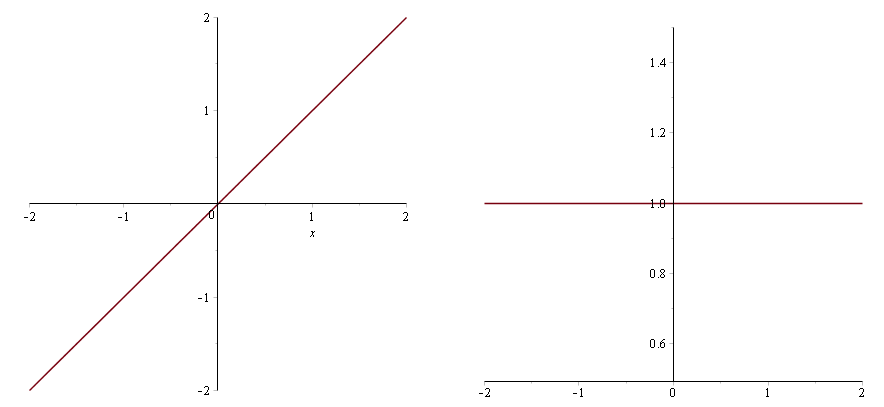
\includegraphics[width=0.6\linewidth]{images/2_linear}
 \caption[Lineare Aktivierungsfunktion und ihre Ableitung]{Lineare Aktivierungsfunktion (links) und Ableitung (rechts)}
 \label{fig:2_linear}
 \end{figure}

\begin{itemize}
\item Funktion:  
\begin{equation} 
f(x) =  x 
\end{equation}
\item Ableitung: 
\begin{equation} 
f'(x) = 1 
\end{equation}
\end{itemize}


\subsubsection{Logistische Sigmoidfunktion}
Ein Spezialfall der Sigmoidfunktion ist die logistische Funktion. Diese nichtlineare Funktion bildet $\mathbb{R} \rightarrow (0,1) $ ab (siehe Abbildung \ref{fig:2_sig}). Eine Besonderheit der Sigmoidfunktion ist, dass die Ableitung an einer bestimmten Stelle durch die Funktion selbst berechnet werden kann.

 \begin{figure}[H]
 \centering
 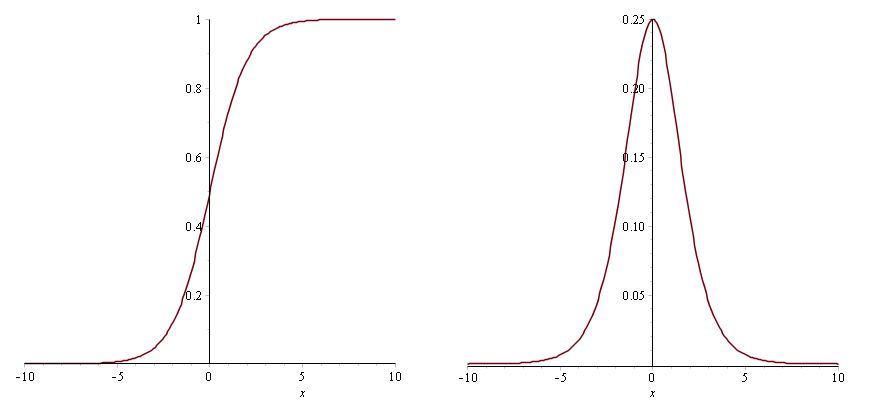
\includegraphics[width=0.6\linewidth]{images/2_sigmoid}
 \caption[Sigmoid Aktivierungsfunktion und Ableitung]{Sigmoid Aktivierungsfunktion (links) und Ableitung (rechts)}
 \label{fig:2_sig}
 \end{figure}
 
 \begin{itemize}
 \item Funktion: 
  \begin{equation} 
 sig(x) = \frac{1}{1 + \exp^{-t}}  
 \end{equation}
 \item Ableitung: 
 \begin{equation} 
 sig'(x) = sig(x)(1-sig(x))
 \end{equation}
 \end{itemize}

\subsubsection{Tangens Hyperbolicus}
Die Tangens Hyperbolicus-Funktion ist eine nichtlineare Funktion, welche $\mathbb{R} \rightarrow (-1,1) $ abbildet (siehe Abbildung \ref{fig:2_tanh}). Wie bei der Sigmoidfunktion, kann die Ableitung an einer bestimmten Stelle ebenfalls durch die Funktion selbst berechnet werden.

 \begin{figure}[H]
 \centering
 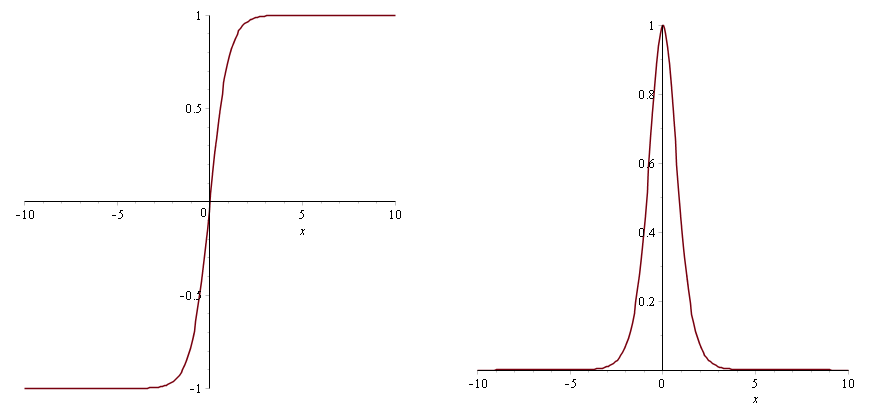
\includegraphics[width=0.6\linewidth]{images/2_tanh}
 \caption[Tangens Hyperbolicus (tanh) Aktivierungsfunktion und Ableitung]{Tangens Hyperbolicus (tanh) Aktivierungsfunktion (links) und Ableitung (rechts)}
 \label{fig:2_tanh}
 \end{figure}
 
  \begin{itemize}
  \item Funktion: 
	  \begin{equation} 
	  tanh(x) = \frac{\exp^x - \exp^{-x}}{\exp^x + \exp^{-x}} 
	  \end{equation}
  \item Ableitung: 
  \begin{equation} 
  	tanh'(x) =1 - tanh(x)^2 
  	\end{equation}
  \end{itemize}

\subsubsection{Rectified Linear}
Die \textit{Rectified Linear}-Funktion (ReLu) ist eine von \cite{Glorot2011} eingeführte Aktivierungsfunktion mit Eigenschaften, die im Bereich der Neuronalen Netze von Interesse sind. So ist bei dieser Aktivierungsfunktion für alle Werte, welche eine von 0 verschiedene Ausgabe erzeugen auch die Ableitung von 0 verschieden. Außerdem können keine negativen Werte auftreten. Die Funktion bildet $\mathbb{R} \rightarrow [0,\infty) $ ab und ist in Abbildung \ref{fig:2_relu} dargestellt.

 \begin{figure}[H]
 \centering
 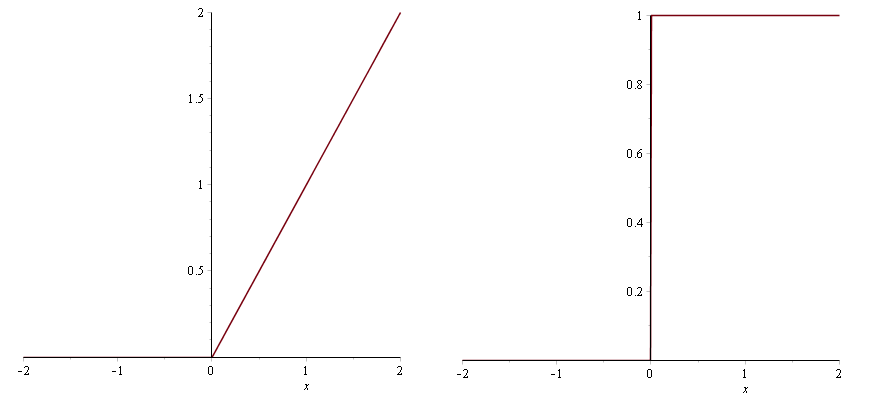
\includegraphics[width=0.6\linewidth]{images/2_relu}
 \caption[Rectified Linear (ReLu) Aktivierungsfunktion und Ableitung]{Rectified Linear (ReLu) Aktivierungsfunktion (links) und Ableitung (rechts)}
 \label{fig:2_relu}
 \end{figure}
 
   \begin{itemize}
   \item Funktion: 
   			\begin{equation} 
   			f(x) =  max(0,x) 
   			\end{equation}
   \item Ableitung: 
   		\begin{equation}
   		   f'(x) =
   		   \begin{cases}
   		     0 & \text{f"ur } 0 \ge x  \\
   		     1 & \text{f"ur } 0 < x
   		     \end{cases}
   		\end{equation}
   \end{itemize}
 

\subsubsection{Softplus}
Die \textit{Softplus}-Funktion ist eine glatte Variante der ReLu-Funktion, welche
 $\mathbb{R} \rightarrow (0,\infty) $ abbildet. Die \textit{Softplus}-Funktion ist in Abbildung \ref{fig:2_sofplus} dargestellt.

 \begin{figure}[H]
 \centering
 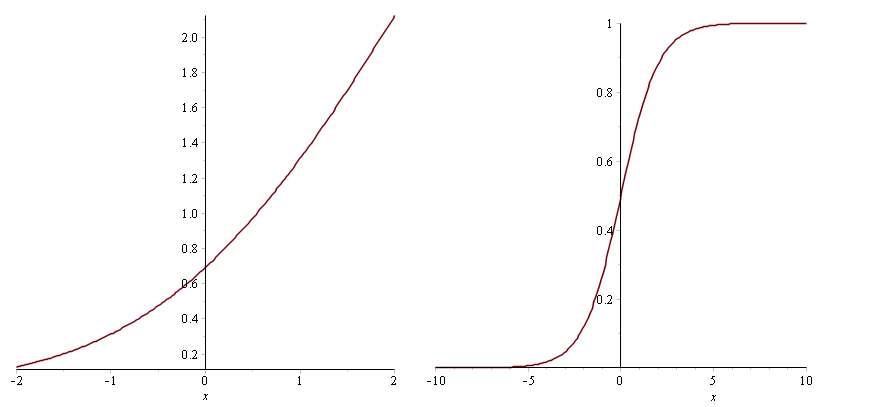
\includegraphics[width=0.6\linewidth]{images/2_softplus}
 \caption[Softplus Aktivierungsfunktion und Ableitung]{Softplus Aktivierungsfunktion (links) und Ableitung (rechts)}
 \label{fig:2_sofplus}
 \end{figure}

 
   \begin{itemize}
   \item Funktion:  
   		\begin{equation} 
   		f(x) =  ln(1+\exp^x) 
   		\end{equation}
   \item Ableitung: 
   	\begin{equation} 
   	f'(x) = \frac{1}{1+\exp^{-x}}
   	\end{equation}
   \end{itemize}

\section{Fehlermaße}
Feedforward-Netze basieren auf dem sogenannten \textit{Error-Correction Learning}. Das bedeutet, dass das Ausgabesignal $y_k$ eines Neuron $k$ (\textit{Output}) des Netzwerks zu einem Eingangssignal $x$ mit einem Zielsignal $d_k$ (\textit{Target})  verglichen und so das Fehlersignal $e_k = d_k - y_k$ erzeugt wird \cite[vgl.][S. 51f]{Haykin1999}.

Um das Fehlersignal in MLPs zu messen, wird ein entsprechendes Fehlermaß benötigt. Dabei werden meist der Mittlere Quadratische Fehler (\textit{Mean Squared Error}) für Regression- und die negative Log-Likelihood (\textit{Cross-Entropy}) für Klassifikationsaufgaben verwendet \cite[vgl.][]{Golik2013}. 

\subsection{Mittlerer Quadratischer Fehler}
Der \textit{Mean Squared Error} (MSE) ist für ein gegebenes MLP $f(x)$ und gegebene Trainingsdaten $D = \{(x_1,y_1),..(x_n,_n)\}$ wie in Gleichung \ref{eq:mse} definiert. Eine Besonderheit stellt der zusätzliche Faktor $\frac{1}{2}$ dar, welcher letztlich aber nur die Ableitung vereinfacht.

 	\begin{equation} 
 	\label{eq:mse}
   	MSE = \frac{1}{2N}\sum_{i}^{N}(f(x_i) - y_i)^2	
   	\end{equation}

\subsection{Cross-Entropy}
Das \textit{Cross-Entropy}-Fehlermaß (CE) ist in Gleichung \ref{eq:cross} dargestellt. Es beschreibt die negative Log-Likelihood über den gesamten Trainingsdaten $D = \{(x_1,y_1),..(x_n,_n)\}$ \cite[vgl.][S. 118]{Mitchell1997}. Als Vorgriff auf Kapitel \ref{ch:gradient} wird hier bereits CE über die Trainingsdaten gemittelt angegeben.

\begin{equation} 
 	\label{eq:cross}
   	CE = - \frac{1}{N}\sum_{i}^{N}(y_i ln(f(x_i)) + (1 - y_i) ln(1 - f(x_i))	
   	\end{equation}

Durch die $ln(\cdot)$-Funktion beachtet CE im Gegensatz zu MSE wie nah das Ausgabesignal am Zielsignal ist, vernachlässigt allerdings im Gegenzug fehlerbehaftete Ausgaben. Dieser Zusammenhang trägt dazu bei, dass CE für Klassifikationsaufgaben besser geeignet erscheint. 


\section{Backpropagation-Algorithmus}
\label{ch:backprop}
In den vergangenen Kapiteln wurden, ausgehend vom Perzeptron, die nichtlinearen MLPs eingeführt und verschiedene Aktivierungsfunktionen vorgestellt. Außerdem wurde gezeigt, dass der Fehler eines Neuronalen Netzes mittels zwei verschiedenen Fehlermaßen angegeben werden kann. Wie im vergangenen Kapitel festgestellt wurde, wird bei Neuronalen Netzen ein sogenanntes \textit{Error-Correction Learning} angewandt. Dazu ist es nötig formal eine Regel zu definieren, mit welcher die Gewichte des Netzwerks verändert werden, um die Performance hinsichtlich des gewählten Fehlermaßes zu optimieren (Gradientenverfahren): Die sogenannte Delta-Regel (vgl. \cite{Widrow1960} und \cite{Widrow1988}. 

Für das Anpassen der Gewichte und Schwellwerte in einem MLP mit nichtlinearen Aktivierungsfunktionen wird eine Verallgemeinerung, der von \cite{Rumelhart1986a} entwickelte Backpropagation-Algorithmus, verwendet. Dieser besteht abstrakt gesehen aus zwei Phasen. In der ersten Phase wird die Ausgabe des Netzes sowie der entsprechende Fehler berechnet (\textit{Forward Pass}), in der zweiten der Fehler mittels Delta-Regel zurück propagiert und so der Gradient schichtweise durch Anwendung der Kettenregel berechnet (\textit{Backward Pass}).

Im Folgenden wird der Backpropagation-Algorithmus vorgestellt \cite[vgl. z.B.][S. 151 ff.]{Rojas1996}. Beispielhaft dient hier der MSE als Fehlermaß.


\begin{multicols}{2}
\begin{itemize}
\item $W^l$: Gewichtsmatrix
\item $b^l$: Vektor mit Schwellwerten
\item $J(\cdot)$: Kostenfunktion
\item $x$: Eingabevektor
\item $x^l$: Layer-Eingabevektor 
\item $f(\cdot)$: Ausgabevektor
\item $\phi(\cdot)$: Aktivierungsfunktion
\item $z^l$: Linearer Ausgabevektor
\item $a^l$: Aktivierter Ausgabevektor
\item $N$: Anzahl Trainingsbeispiele
\item $L$: Anzahl Layer
\item $\circ$: Hadamard-Produkt
\item $\eta$: Lernrate
\end{itemize}
\end{multicols}

Gleichung \ref{eq:backprop0} definiert die Kostenfunktion:
\begin{equation} 
\label{eq:backprop0}
J(W,b) = \frac{1}{2N} \sum_{i=1}^{N}(f(x_i) - y_i)^2	
\end{equation}

Die Gleichungen \ref{eq:backprop1} und \ref{eq:backprop2} beschreiben den allgemeinen Gradientenabstieg:
\begin{equation} 
\label{eq:backprop1}
W_{t+1}^l = W_t - \eta {\nabla W_t} %\frac{1}{N} \sum_{i=1}^{N} \frac{\partial J(W_t,b_t)}
\end{equation}

\begin{equation} 
\label{eq:backprop2}
b_{t+1}^l = b_t - \eta {\nabla b_t} %\frac{1}{N} \sum_{i=1}^{N} \frac{\partial J(W_t,b_t)}
\end{equation}

Der Backpropagation-Algorithmus kombiniert die Delta-Regel mit der Kettenregel und beschreibt so ein Verfahren zur Berechnung der Ableitungen von zusammengesetzten Funktionen. Es wird somit der Gradient für jede Schicht des MLP iterativ berechnet. Um den Gradienten der Kostenfunktion $\nabla J(W,b)$ zu berechnen, wird zuerst für jedes Trainingsbeispiel $\nabla J(W,b,x_i,y_i)$ einzeln berechnet und aufsummiert. Folgende Formeln \ref{eq:backprop3} und \ref{eq:backprop4} beschreiben die Delta-Regeln des Backpropagation-Algorithmus: \\

Delta Output-Layer:
\begin{equation} 
\label{eq:backprop3}
\delta^{L} = (a_i^{L} - y_i) \circ \phi'(z^{L})
\end{equation}

Delta für Hidden-Layer $l$:
\begin{equation} 
\label{eq:backprop4}
\delta^{l} =  ((W^{l+1})^T\delta^{l+1}) \circ \phi'(z^l)
\end{equation}

Die partiellen Ableitungen pro Schicht (Gleichung \ref{eq:backprop5} und \ref{eq:backprop6}) werden über alle Trainingsbeispiele $1..N$ aufsummiert und am Ende eines Durchlaufs mit $\frac{1}{N}$ gemittelt. \\

Partielle Ableitung für Layer $l$:
\begin{equation} 
\label{eq:backprop5}
\frac{\partial J(W,b)}{\partial W^l} = \frac{1}{N} \sum_{i=1}^{N} \delta^{l} (x_i^{l})^T
\end{equation}

\begin{equation} 
\label{eq:backprop6}
\frac{\partial J(W,b)}{\partial b^l} = \frac{1}{N} \sum_{i=1}^{N} \delta^{l}
\end{equation}

Betrachtet man die Delta-Formeln \ref{eq:backprop3} und \ref{eq:backprop4}, wird ersichtlich, dass sich die Verwendung einer Aktivierungsfunktion, deren Ableitung sich durch den Funktionswert selbst berechnen lässt, besonders eignet. Im Falle der Sigmoid-Funktion vereinfacht sich $\phi'(z^l)$ so zu $sig'(z^l) = sig(a^l)(1-sig(a^l))$, was das Speichern von $z^l$ erübrigt.


% Hakin heranführung delta rule	
%	- Backpropagation for gradient computation 			(1 Seite)
%		- derivative of weighting matrix
% 	- Von LMS tu Backpropagation
%   - Beispiel Kettenregel
%Backpropagation ROjas Kaptitel
%
%Bilder
%http://galaxy.agh.edu.pl/~vlsi/AI/backp_t_en/backprop.html



\section{Basisarchitekturen}
Dieses Kapitel beschreibt die zwei Grundarchitekturen Neuronaler Netze (MLPs). Diese umfassen einerseits die  Softmax-Regression zur Klassifikation und andererseits die Nicht\-lineare-Regression.
		
\subsection{Softmax-Regression (Klassifikation)}
\label{ch:softmax}
Die Logistische Regression stellt ein bekanntes lineares statistisches Regressi\-onsverfahren zur Modellierung diskreter abhängiger Variablen dar, welches ursprünglich nichts mit dem Neuronalen Lernmodell zu tun hat. Praktischerweise entspricht dieses jedoch der gleichen Architektur, was die Verwendung als Ausgabeschicht für die Klassifikation mit MLPs nahelegt. Abbildung \ref{fig:2_logistic_regression} zeigt das Verfahren für die diskreten Werte 0 und 1, wobei die Hyperebene zur Visualisierung um $0.5$ verschoben ist.

Allgemein wird mittels des Verfahrens, bei gegebenen Gewichten $W$, die Wahrscheinlichkeit einer binären Ausgabe $y_i \epsilon \{0 ,1\}$ für eine gegebene Eingabe $x_i$ berechnet \cite[vgl. z. B.][S. 119 ff.]{Hastie2009}. 
Die Güte des Models über den gesamten Trainingsbeispielen $N$ kann mit der Formel \ref{eq:logisticRegression} bestimmt werden. Zur Vereinfachung wird von erweiterten Gewichtsvektoren $\hat{w}$ ausgegangen, in denen der Schwellwert $b$ integriert ist.

\begin{figure}
\centering
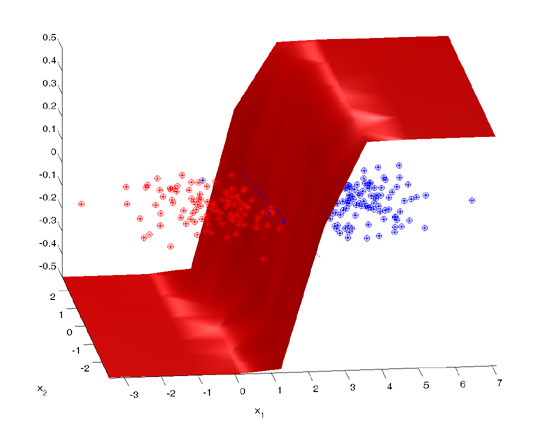
\includegraphics[width=0.5\linewidth]{images/2_logistic_regression}
\caption[Logistische Regression mit zwei Klassen]{Logistische Regression mit zwei Klassen (Bild: Vadim Strijov, Computing Centre of the Russian Academy of Sciences)}
\label{fig:2_logistic_regression}
\end{figure}


\begin{equation} 
\label{eq:logisticRegression}
p(y|X,\hat{W}) = \prod_{i=1}^N [\frac{1}{1 + \exp^{-\hat{W}x_i}} ]^{y_i}  [1 - \frac{1}{1 + \exp^{-\hat{W}x_i}} ]^{1-y_i}
\end{equation}

Wird nun die Likelihood maximiert beziehungsweise die negative Log-\-Likeli\-hood minimiert, erhält man die Formel \ref{eq:logisticRegression2} mit $f(x_i) = \frac{1}{1 + \exp^{-\hat{W}x_i}} $. Dies entspricht proportional einem einschichtigen MLP mit Sigmoid-Akti\-vierungs\-funktion sowie \textit{Cross-Entropy}-Fehlermaß und lässt sich somit mittels des Back\-propa\-gation-Algorithmus optimieren. 

\begin{equation} 
\label{eq:logisticRegression2}
- ln(p(y|X,\hat{W})) = - \sum_{i=1}^N  y_i ln(f(x_i)) + (1-y_i) ln(1 - f(x_i))
\end{equation}


\subsubsection{Multinomiale Regression}
Mehrdimensionale Ausgaben können in neuronalen Netzen durch einfaches Hinzufügen von Neuronen zum Output-Layer erzeugt werden. 
Ein gern verwendeter Code, um mehrere Klassen darzustellen, ist der sogenannte \textit{Grand\-mother-Cell}-Code \cite[vgl.][]{LeCun1998}. Hier wird für $d$-Klassen ein $d$-dimensionaler Zielvektor oder erweiterter Labelvektor definiert mit $d_j = 1$ für die Klasse $j$.
Das Modell der Logistischen Regression lässt sich ebenso leicht auf mehrere Klassen erweitern. Dazu muss die Ausgabe, um ein valides probabilistisches Modell zu erhalten, normalisiert werden. Gleichung \ref{eq:logisticRegression3} beschreibt die Kostenfunktion der multinomialen Regression. Diese ist im Bereich Neuronale Netze eher bekannt als Softmax-Regression (vgl. z.B. \cite{Krizhevsky2012} und \cite{Bengio2015}).

\begin{equation} 
\label{eq:logisticRegression3}
- ln(p(y|X,\hat{W})) = - \sum_{i=1}^N  \sum_{j=1}^d 1\{y^i = j \} ln[\frac{\exp^{\hat{w}_j^Tx^i}}{\sum_{l=1}^d\exp^{\hat{w}_l^Tx^i}} ]
\end{equation}


Neben der Softmax-Regression wird teilweise auch ein Output-Layer mit radialen Basisfunktionen (RBFs) verwendet \cite[vgl.][]{LeCun1998}. Dies hat den Vorteil, dass für jede Klasse ein eigener spezifischer Labelvektor definiert werden kann. Ein Nachteil ist jedoch, dass diese Variante die Ausgabe nicht normalisiert und somit nicht probabilistisch interpretiert werden kann. 
Als Basisfunktionen im Hidden-Layer eignen sich RBFs nur sehr bedingt, da diese lokal im Eingaberaum sind und daher sehr viele Einheiten für hochdimensionale Räume benötigt werden \cite[vgl.][]{LeCun1998b}.

\subsubsection{Besonderheit in Verbindung mit Backpropagation}
Wird Backpropagation angewandt, muss im Output-Layer die Ableitung der Aktivierungsfunktion berechnet werden. Gleichung \ref{eq:softmax} zeigt diese für die Softmax-Funktion. $\delta$ entspricht hierbei dem Kronecker-Delta.
\begin{equation} 
\label{eq:softmax}
softmax'(x)_{ij} = softmax(x)_i(\delta_{ij} - softmax(x)_j)
\end{equation}

Dieser Ausdruck ist sehr unhandlich. Es lässt sich allerdings zeigen, dass die Softmax-Regression in Verbindung mit einem \textit{Cross-Entropy}-Fehlermaß die Berechnung von $\delta^L$ nicht erschwert, sondern zu Gleichung \ref{eq:softmax2} vereinfacht  \cite[vgl. z. B.][Kap. 6.3.2, S. 167]{Bengio2015}. \\

Delta Output-Layer:
\begin{equation} 
\label{eq:softmax2}
\delta^{L} = a_i^{L} - y_i
\end{equation}

Dies bietet damit den großen Vorteil, dass $\delta^L$ nur noch vom Fehler abhängt und nicht mehr von der Ableitung der Aktivierungsfunktion und damit die Nichtlinearität am Ausgang nicht gesättigt wird.


\subsection{Funktionsapproximation (Regression)}
Neuronale Netze können beliebige Funktionen $f:\mathbb{R}^n \rightarrow \mathbb{R}^m $ approximieren und so mittels Backpropagation auf beliebige Daten trainiert werden \cite[vgl.][S. 269 ff.]{Rojas1996}. Es ist lediglich darauf zu achten, dass der Wertebereich des Output-Layers zu dem der Labels passt. So werden im Output-Layer meist lineare Aktivierungsfunktionen verwendet. Alternativ können auch die Labels auf den Wertebereich der verwendeten Aktivierungsfunktion skaliert werden.

\begin{figure}
\centering
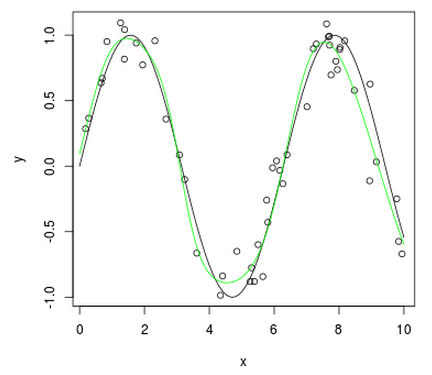
\includegraphics[width=0.5\linewidth]{images/2_sine_nn}
\caption[Approximierte Sinuskurve mit einem Hidden-Layer mit 6 Neuronen (grün)]{Approximierte Sinuskurve mit einem Hidden-Layer mit 6 Neuronen (grün)}
\label{fig:2_sine}
\end{figure}

Abbildung \ref{fig:2_sine} zeigt eine Sinuskurve, welche von einem MLP mit 6 Neuronen im Hidden-Layer approximiert wird. Die zugrundeliegende Trainingsdaten sind aus einer Sinuskurve mit additivem normalverteilten Rauschen generiert. 

